% IF YOU CAN SEE THIS GO CONTRIBUTE >:(

\documentclass[letterpaper, 8pt]{extarticle}
\usepackage{amssymb,amsmath,amsthm,amsfonts}
\usepackage{multicol,multirow}
\usepackage{calc}
\usepackage{ifthen}
\usepackage[landscape]{geometry}
\usepackage[colorlinks=true,citecolor=blue,linkcolor=blue]{hyperref}

\usepackage{booktabs}
\usepackage{ulem}
\usepackage{enumitem}
\usepackage{tabulary}
\usepackage{graphicx}
\usepackage{siunitx}
\usepackage{tikz}
\usepackage{derivative}
\usepackage{svg}
\usepackage{listings}
\usepackage{setspace}
\usepackage{listings}
\usepackage{xcolor}
\usepackage{courier}
\usepackage{syntax}
\usepackage{mathpartir}
\usepackage{siunitx}

% minimal line spacing
% \setstretch{0.1}

% set borders (experimentally determined to minimize cutoff and maximize space on school printers)
\geometry{top=.25in,left=.25in,right=.25in,bottom=.35in}

% make figures work better in multicol
\newenvironment{Figure}
{\par\medskip\noindent\minipage}
{\endminipage\par\medskip}

\pagestyle{empty} % clear page

% rewrite section commands to be smaller
\makeatletter
\renewcommand{\section}{\@startsection{section}{1}{0mm}%
                                {-1explus -.5ex minus -.2ex}%
                                {0.5ex plus .2ex}%x
                                {\normalfont\small\bfseries}}
\renewcommand{\subsection}{\@startsection{subsection}{2}{0mm}%
                                {-1explus -.5ex minus -.2ex}%
                                {0.5ex plus .2ex}%
                                {\normalfont\tiny\bfseries}}
\renewcommand{\subsubsection}{\@startsection{subsubsection}{3}{0mm}%
                                {-1ex plus -.5ex minus -.2ex}%
                                {1ex plus .2ex}%
                                {\normalfont\tiny\bfseries\itshape}}
\makeatother
\setcounter{secnumdepth}{0} % disable section numbering


% disable indenting
\setlength{\parindent}{0pt}
\setlength{\parskip}{0pt plus 0.5ex}

% Custom siunitx defs
\DeclareSIUnit\noop{\relax}
\NewDocumentCommand\prefixvalue{m}{%
\qty[prefix-mode=extract-exponent,print-unity-mantissa=false]{1}{#1\noop}
}

% Shorthand definitions
\newcommand{\To}{\Rightarrow}
\newcommand{\ttt}{\texttt}
\newcommand{\ra}{\rightarrow}

% condense itemize & enumerate
\let\olditemize=\itemize \let\endolditemize=\enditemize \renewenvironment{itemize}{\olditemize \itemsep0em}{\endolditemize}
\let\oldenumerate=\enumerate \let\endoldenumerate=\endenumerate \renewenvironment{enumerate}{\oldenumerate \itemsep0em}{\endoldenumerate}
\setlist[itemize]{noitemsep, topsep=0pt, leftmargin=*}
\setlist[enumerate]{noitemsep, topsep=0pt, leftmargin=*}

\title{3GC3}

\begin{document}
\raggedright
\tiny

% make listings look nicer
\lstset{
    tabsize = 2, %% set tab space width
    showstringspaces = false, %% prevent space marking in strings, string is defined as the text that is generally printed directly to the console
    basicstyle = \tiny\ttfamily, %% set listing font and size
    breaklines = true, %% enable line breaking
    numberstyle = \tiny,
    postbreak = \mbox{\textcolor{red}{\(\hookrightarrow\)}\space}
}

\begin{center}
    {\textbf{3GC3 Final - RTX ON Edition}} \\
\end{center}
% set column spacing rules
\setlength{\premulticols}{1pt}
\setlength{\postmulticols}{1pt}
\setlength{\multicolsep}{1pt}
\setlength{\columnsep}{2pt}
\begin{multicols*}{4}

\section{Math}
\textbf{Dot Product}:
\(
\mathbf{a} \cdot \mathbf{b}
= x_a x_b + y_a y_b + z_a z_b
= ||\mathbf{a}|| ||\mathbf{b}|| \cos \phi
\)

\textbf{Cross Product}:
\(
\mathbf{a} \times \mathbf{b}
= (y_a z_b - z_a y_b, z_a x_b - x_a z_b, x_a y_b - y_a x_b)
= ||\mathbf{a}|| ||\mathbf{b}|| \sin(\theta) \mathbf{n}
\)

\textbf{MatMul}:\\
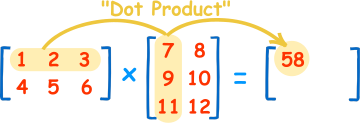
\includegraphics[width=0.5\linewidth]{matrix-multiply-a.png}
For target $c_{i,j}$ iterate over the $i$th row in the first matrix and the $j$th column in the second -- perform inner product and save.

\textbf{Right Hand Rule}:
For axises, $x$ is thumb, $y$ is index, and $z$ is middle finger.

\textbf{Interpolation}:
\(t\) is how far along the line \(p_t\) is from \(p_0\) to \(p_1\) as a percentage between 0 and 1.
\(
t = (x_t - x_0) / (x_1 - x_0)
\text{ or }
t = (y_t - y_0) / (y_1 - y_0)
\)
\(
v_t = (1-t) v_0 + t v_1
\)

\textbf{Bi-linear Interpolation}
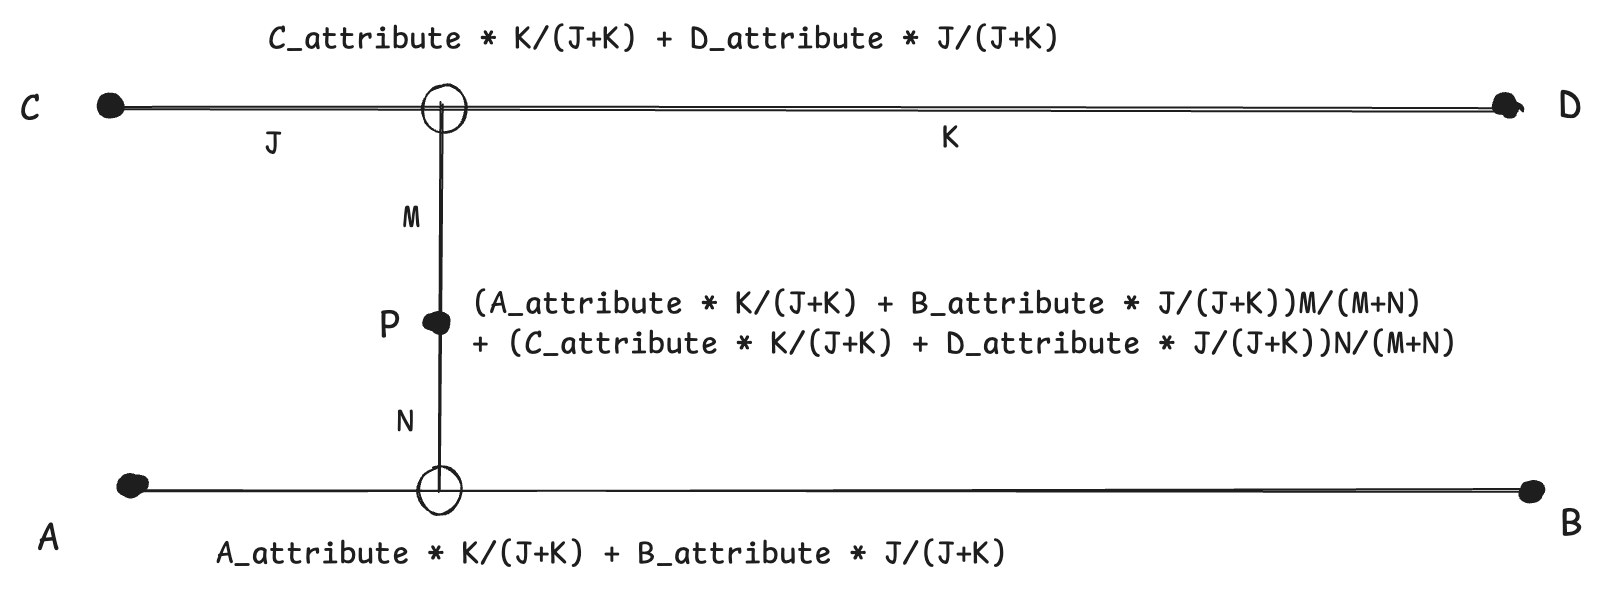
\includegraphics[width=4cm]{bilinear-interpolation.png}

\textbf{Cramer's Rule}
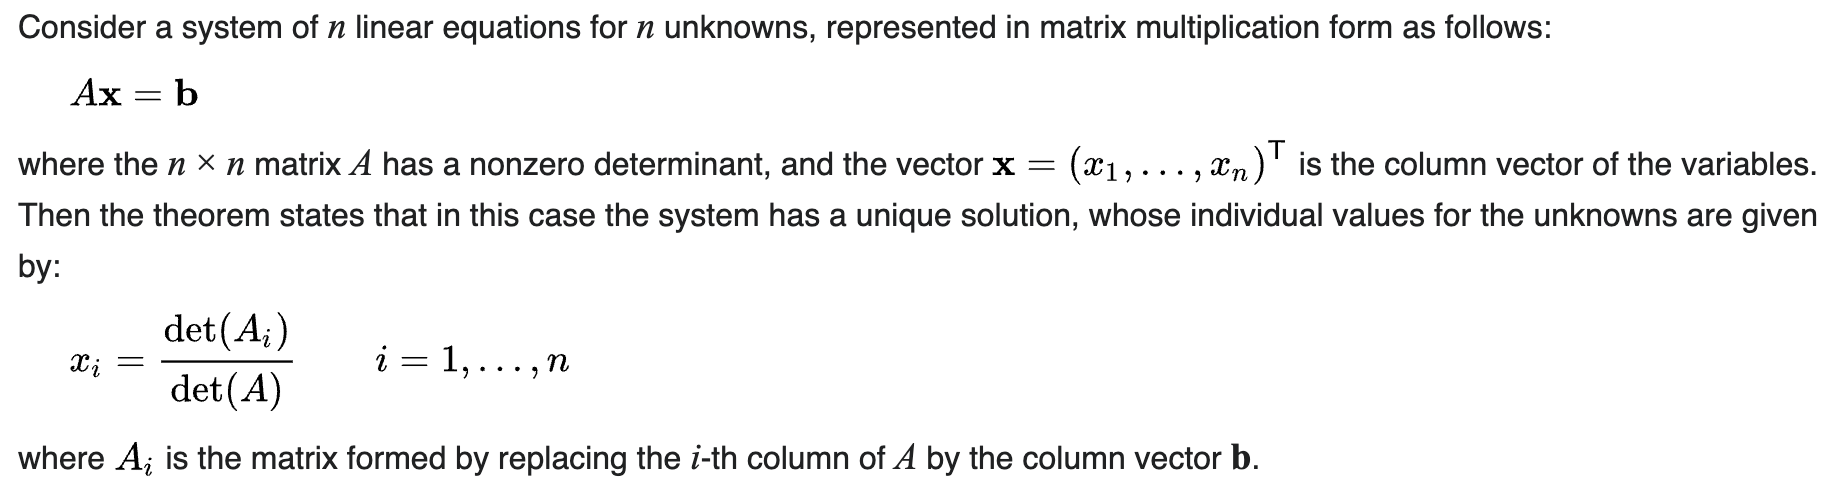
\includegraphics[width=4cm]{cramer.png}

\textbf{Barycentric Interpolation (Area)}:
From Triangle ABC, point $P(x,y,z)$ can be defined using $u,v,w$, where $P = uA + vB + wC$. \textbf{IMPORTANT:} $u + v + w = 1$.

From World to Bary: 
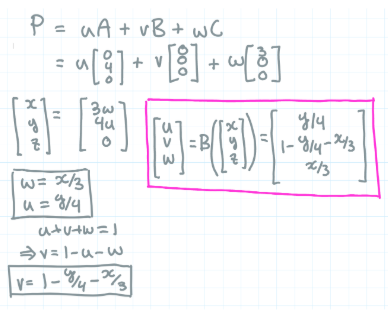
\includegraphics[width=0.8\linewidth]{bary-transform.png}


% \textbf{Barycentric Interpolation (Area)}:
% \(
% \alpha = A_a / A \quad
% \beta = A_b / A \quad
% \gamma = A_c / A \quad
% s.t.\ \alpha + \beta + \gamma = 1
% \)

% Now,
% \(
% \mathbf{p}(\alpha, \beta, \gamma)
% = \alpha \mathbf{a} + \beta \mathbf{b} + \gamma \mathbf{c}
% \)

% \textbf{Barycentric Interpolation (line function)}:
% $f_{ij}(x, y) = (y_i - y_j) x + (x_j - x_i)y + x_i y_j - x_j y_i$ \\
% $\alpha = \frac{f_{bc}(x_P, y_P)}{f_{bc}(x_a, y_a)},\
% \beta = \frac{f_{ac}(x_P, y_P)}{f_{bc}(x_b, y_b)},\
% \gamma = \frac{f_{ab}(x_P, y_P)}{f_{ab}(x_c, y_c)}$

\section{Transformations \& Coordinate Systems}
\textbf{Linear Transformation}:
\(
f(\begin{bmatrix}
    x \\ y
\end{bmatrix})
= \begin{bmatrix}
    a_{11} & a_{12} \\
    a_{21} & a_{22}
\end{bmatrix}
\begin{bmatrix}
    x \\ y
\end{bmatrix}
=
\begin{bmatrix}
    a_{11} x + a_{12} y \\
    a_{21} x + a_{22} y
\end{bmatrix}
\)
satisfies: \(
f(\mathbf{u} + \mathbf{v})
= f(\mathbf{u}) + f(\mathbf{v})
\)
and
\(
f(c\mathbf{u}) = cf(\mathbf{u})
\)

In other words, origin is unchanged, straight lines remain straight lines.

\textbf{Affine Transformation}
Straight lines remain lines.

\textbf{2D Rotations}
\(
f(p)
= x \begin{bmatrix}
    \cos \theta \\ \sin \theta
\end{bmatrix}
+ y \begin{bmatrix}
    -\sin \theta \\ \cos \theta
\end{bmatrix}
= \begin{bmatrix}
    \cos \theta & - \sin \theta \\
    \sin \theta & \cos \theta
\end{bmatrix}
\begin{bmatrix}
    x \\ y
\end{bmatrix}
\)

\textbf{3D Rotations} \\
Note: All orthonormal matrices are rotation matrices. \\
\textit{Rotate around X}
\(
f(p) = \begin{bmatrix}
    1 & 0           & 0            \\
    0 & \cos \theta & -\sin \theta \\
    0 & \sin \theta & \cos \theta
\end{bmatrix}
\begin{bmatrix}
    x \\ y \\ z
\end{bmatrix}
\)

\textit{Rotate around Y}
\(
f(p) = \begin{bmatrix}
    \cos \theta  & 0 & \sin \theta \\
    0            & 1 & 0           \\
    -\sin \theta & 0 & \cos \theta
\end{bmatrix}
\begin{bmatrix}
    x \\ y \\ z
\end{bmatrix}
\)

\textit{Rotate around Z}
\(
f(p) = \begin{bmatrix}
    \cos \theta & -\sin \theta & 0 \\
    \sin \theta & \cos \theta  & 0 \\
    0           & 0            & 1
\end{bmatrix}
\begin{bmatrix}
    x \\ y \\ z
\end{bmatrix}
\)

For a generic 3D rotation:
\(
R =
\begin{bmatrix}
    ax & bx & cx \\
    ay & by & cy \\
    az & bz & cz
\end{bmatrix}
\)
Where the \(a*\) column is the coordinates of the object's \(x'\) vector,
the \(b*\) column is the \(y'\) vector,
and the \(c*\) column is the \(z'\) vector:
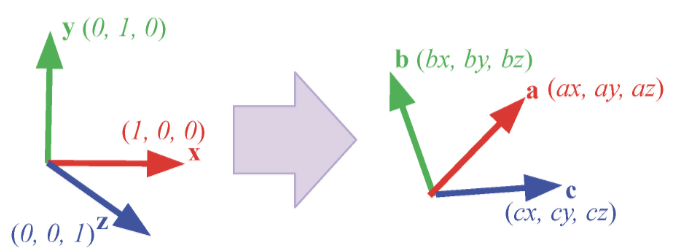
\includegraphics[width=4cm]{3d-rotation.png}

\textbf{2D Reflection}
Reflect X:\@
\(
\begin{bmatrix} -1 & 0 \\ 0 & 1 \end{bmatrix}
\)
Reflect Y:\@
\(
\begin{bmatrix} 1 & 0 \\ 0 & -1 \end{bmatrix}
\)

\textbf{3D Scaling}
\(
\begin{bmatrix}
    s_x & 0   & 0   \\
    0   & s_y & 0   \\
    0   & 0   & s_z
\end{bmatrix}
\begin{bmatrix}
    x \\ y \\ z
\end{bmatrix}
=
\begin{bmatrix}
    s_x x \\ s_y y \\ s_z z
\end{bmatrix}
\)

% \textbf{2D Shear Matrix}
% Horizontal shear (top edge is shifted to the right (positive)):
% \(
% \begin{bmatrix}
%     1 & s_x \\
%     0 & 1
% \end{bmatrix}
% \)
% Vertical shear (right edge is shifted up (positive)):
% \(
% \begin{bmatrix}
%     1   & 0 \\
%     s_y & 1
% \end{bmatrix}
% \)

% \textbf{3D Shear Matrix}
% 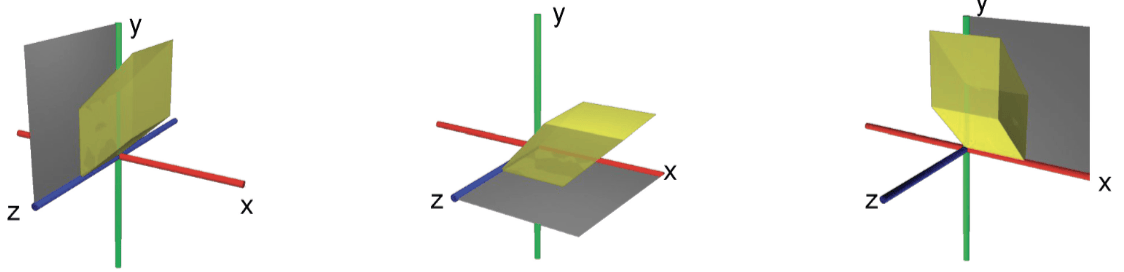
\includegraphics[width=4cm]{3d-shear.png}
% Shear on YZ Plane:
% \(
% \begin{bmatrix}
%     1   & 0 & 0 \\
%     s_y & 1 & 0 \\
%     s_z & 0 & 1
% \end{bmatrix}
% \)

% Shear on XZ Plane:
% \(
% \begin{bmatrix}
%     1 & s_x & 0 \\
%     0 & 1   & 0 \\
%     0 & s_z & 1
% \end{bmatrix}
% \)

% Shear on XY Plane:
% \(
% \begin{bmatrix}
%     1 & 0 & s_x \\
%     0 & 1 & s_y \\
%     0 & 0 & 1
% \end{bmatrix}
% \)

\textbf{Homogenous Coordinate}
2D points represented by \((x, y, z)\), 2D location is \((x/z, y/z) \mid z=1\) or other value
3D points represented by \((x, y, z, w)\), 3D location is \((x/w, y/w, z/w) \mid w=1\) or other value
Used for perspective projection, \(z\) becomes depth value.

\textit{Transformation Matrix}
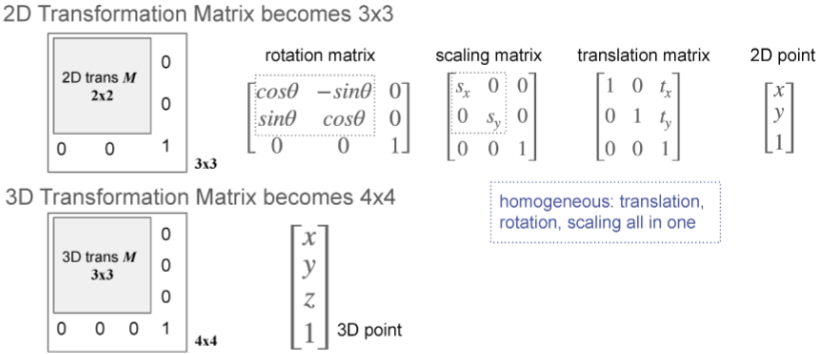
\includegraphics[width=\linewidth]{homogenous-coord-transformation-matrix.png}

\textbf{Composite Transformation}
Since scaling, rotation, etc is about origin, operations are not commutive!

\textit{Examples}
To rotate around an object's centre, 1 translate object centre to origin, 2 rotate, 3 translate back.

To scale an object along a non uniform axis, 1 rotate the object to align with a canonical axis, 2 scale object, 3 rotate object back.

\textbf{Inversions}
For rotation, scaling, and translating,
the inverse of a matrix \(M^{-1}\) can be used.
For rotation specifically, \(M^{-1}_{rotate}=M^T_{rotate}\)
For scaling, inversion is essentially \(1/s\) for your scale factor.
For translating, do \(-x\).

\textbf{Coordinate Systems}
\textit{World/Global Coordinate}
Only one, unique.
Each model in scene goes through \(M_{model}\) to transform from model space to world space.

\section{Camera / Viewing Transformations}
% Rendering steps:
% 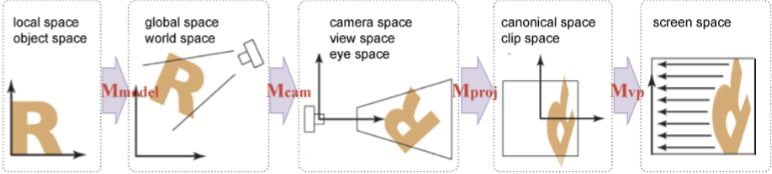
\includegraphics[width=\linewidth]{rendering-steps.png}

% 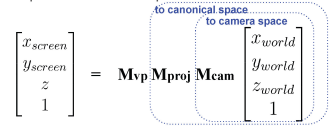
\includegraphics[width=4cm]{cam-total.png}

\textbf{Viewing General Steps}
\begin{enumerate}
    \item Model 3D Objects in local space
    \item Put 3D object at world coordinates
    \item View scene in Camera space
    \item Project camera space into cannonical space
    \item Transform cannonical space to screen
\end{enumerate}

\textbf{World Space $\to$ Camera Space: $M_{cam}$}
Given camera position $e$, gaze direction $g$ and `up' direction $t$, construct basis $uwv$ for camera coordinate system.
$w = - \frac{g}{||g||}, u = \frac{t \times w}{||t \times w||}, v = w \times u$

Remember that OpenGL LookAt Coordinates is Camera Position + Gaze Direction!

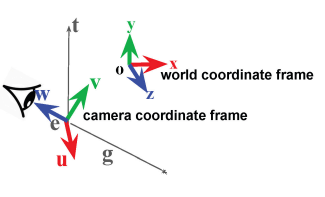
\includegraphics[width=.5\linewidth]{camera-basis.png}

\textit{Camera Space $\to$ World Space:}\\
\(
\begin{bmatrix}
    1 & 0 & 0 & x_e \\
    0 & 1 & 0 & y_e \\
    0 & 0 & 1 & z_e \\
    0 & 0 & 0 & 1   \\
\end{bmatrix}
\)
\(
\begin{bmatrix}
    x_u & x_v & x_w & 0 \\
    y_u & y_v & y_w & 0 \\
    z_u & z_v & z_w & 0 \\
    0   & 0   & 0   & 1 \\
\end{bmatrix}
\)\\

\textbf{World Space $\to$ Camera Space: $M_{cam}=$}\\
\(
\begin{bmatrix}
    x_u & y_u & z_u & 0 \\
    x_v & y_v & z_v & 0 \\
    x_w & y_w & z_w & 0 \\
    0   & 0   & 0   & 1 \\
\end{bmatrix}
\)
\(
\begin{bmatrix}
    1 & 0 & 0 & -x_e \\
    0 & 1 & 0 & -y_e \\
    0 & 0 & 1 & -z_e \\
    0 & 0 & 0 & 1    \\
\end{bmatrix}
\)
\\
Step 1 (left matrix): Translates camera position $e$ to origin $e$. Things originally at $e$ are now at $\vec{0}$.\\
Step 2 (right matrix): Rotates, maps basis vectors: $u \mapsto (1,0,0), v \mapsto (0,1,0), w \mapsto (0,0,1)$

\textbf{3\(\times\)3 Camera Matrix}
\(
M_{cam}
= \begin{bmatrix}
    x_{cam} & y_{cam} & z_{cam}
\end{bmatrix}
\)
Use column vectors

Step 1 (left matrix): Translates camera position $e$ to origin $e$. Things originally at $e$ are now at $\vec{0}$.\\
Step 2 (right matrix): Rotates, maps basis vectors: $u \mapsto (1,0,0), v \mapsto (0,1,0), w \mapsto (0,0,1)$

\textbf{Cannonical Space}\\
Cannonical space is the space $(x, y, z)$ s.t. $x,y,z \in [-1, 1]$.

\textbf{Orthographic Projection}\\

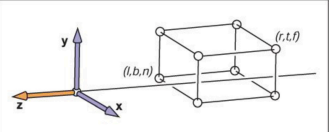
\includegraphics[width=.5\linewidth]{cam-ortho.png}
Given left plane x, $l$, right plane x, $r$, top plane y, $t$, bottom plane y $b$, near plane $n$, far plane $f$.
\textit{Recall that $f$, $n$ are negative z values. See diagram.}

$M_{orth}$ projects the view box defined above onto the canonical space.


$M_{orth}$ = 
%\(
% \begin{bmatrix}
%     \frac{2}{r-l} & 0             & 0             & 0 \\
%     0             & \frac{2}{t-b} & 0             & 0 \\
%     0             & 0             & \frac{2}{n-f} & 0 \\
%     0             & 0             & 0             & 1 \\
% \end{bmatrix}
% \)
% \(
% \begin{bmatrix}
%     1 & 0 & 0 & -\frac{r+l}{2} \\
%     0 & 1 & 0 & -\frac{t+b}{2} \\
%     0 & 0 & 1 & -\frac{n+f}{2} \\
%     0 & 0 & 0 & 1              \\
% \end{bmatrix}
% \)\\
% =
\(
\begin{bmatrix}
    \frac{2}{r-l} & 0             & 0             & -\frac{r+l}{r-l} \\
    0             & \frac{2}{t-b} & 0             & -\frac{t+b}{t-b} \\
    0             & 0             & \frac{2}{n-f} & -\frac{f+n}{n-f} \\
    0             & 0             & 0             & 1                \\
\end{bmatrix}
\)\\
translates center to origin, scales width of all dimensions to be 2, fitting inside [-1, 1].

\textbf{Perspective Projection}\\
% 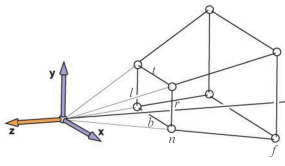
\includegraphics[width=.5\linewidth]{cam-persp.png}
$l,r,b,t$ now define the near plane $XY$, with $n$ being the $Z$. Far plane is only defined by $f$.
\textbf{OR} use depth of field:
$\theta$ = FOV on y-axis, $ratio = (r-l)/(t-b)$, $n$ is near plane z, $f$ is far plane z.

\textbf{Frustrum to Box:}
Recall Homogenous Coordinates. We want frustrum $\mapsto$ box s.t. $n$ stays near and $f$ stays far.

$P$ =
\(
\begin{bmatrix}
    n & 0 & 0   & 0   \\
    0 & n & 0   & 0   \\
    0 & 0 & n+f & -fn \\
    0 & 0 & 1   & 0   \\
\end{bmatrix}
\)\\
$M_{per}$ = $M_{orth}P =$
\(
\begin{bmatrix}
    \frac{2n}{r-l} & 0              & \frac{l+r}{l-r} & 0               \\
    0              & \frac{2n}{t-b} & \frac{b+t}{b-t} & 0               \\
    0              & 0              & \frac{f+n}{n-f} & \frac{2fn}{n-f} \\
    0              & 0              & 1               & 0               \\
\end{bmatrix}
\)\\

\textbf{Cannonical Space To View Port (VP)}\\

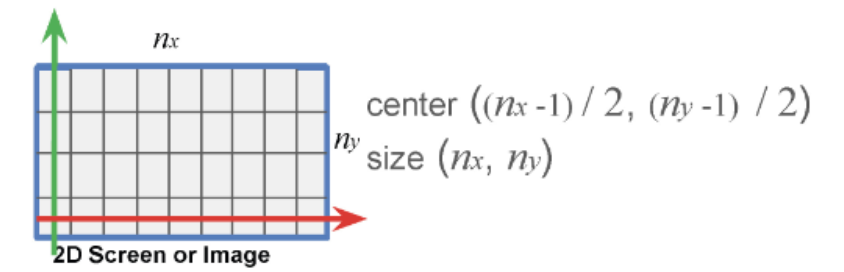
\includegraphics[width=\linewidth]{viewport-diagram.png}
Diagram of viewport, which has no $z$ depth.\\
1. Translate $x,y$ center from $(0,0)$ to $((n_x-1)/2, (n_y-1)/2)$.
2. Scale $x,y$ size from $(2,2)$ to $(n_x, n_y)$.

$M_{vp} = $
\(
\begin{bmatrix}
    \frac{n_x}{2} & 0             & 0 & \frac{n_x-1}{2} \\
    0             & \frac{n_y}{2} & 0 & \frac{n_y-1}{2} \\
    0             & 0             & 1 & 0               \\
    0             & 0             & 0 & 1               \\
\end{bmatrix}
\)\\



\section{Rasterization}

\textit{Definition:} finding all pixels on the screen that are occupied by a geometric primitive.

\textbf{Line Rasterization}
Given pixels $P_0 = (x_0, y_0), P_1 = (x_1, y_1)$, fill the pixels on the screen between them.

$f(x, y): y = mx + c$\\given $m=(y_1 - y_0)/(x_1 - x_0), c=(x_1y_0 - x_0y_1)/(x_1 - x_0)$\\
\textbf{Implicit line function:}: $f(x,y): Ax + By + C = 0$. Checking sign of $f(x_P, y_P)$ can determine point position relative to line. If $A>0 \land B<0$, then $f(x_P, y_P) < 0$ means point $P$ is above the line.\\

\textbf{Naive Implementation:} Use the function $y=mx+c$ and iterate $x$ from $x_0$ to $x_1$. No vertical lines!\\
% \textbf{Digital Difference Analyser DDA:}
% Precomputes step size for both Y and X from line function.
% Marches in direction based on which value changes slower:
% if y changes slower march in the x direction and vice versa.

% 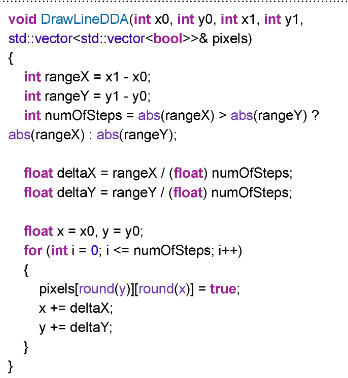
\includegraphics[width=\linewidth]{rasterize-dda.png} 
% \begin{lstlisting}
% drawDDA(p0, p1):
%     ranges = p1-p0
%     numSteps = (ranges.x > ranges.y) 
%         ? ranges.x
%         : ranges.y
%     delta = ranges / numSteps
%     p = p0
%     for i in 0..numSteps:
%         fill pixel (round(p.x), round(p.y))
%         p += delta
% \end{lstlisting}

% \textbf{Bresenham Algorithm:}

% 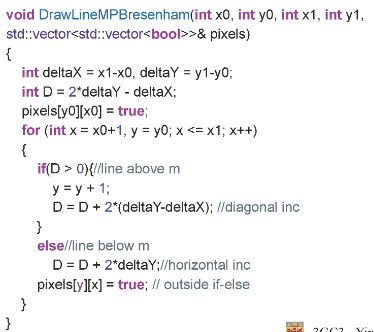
\includegraphics[width=\linewidth]{rasterize-bresen.png}\\
% \begin{lstlisting}
% drawBresenham(x0, y0, x1, y1):
%     deltaX = x1-x0
%     deltaY = y1-y0
%     D = 2*deltaY - deltaX
%     fill pixel (x0,y0)
%     y = y0
%     for x=x0+1; x<=x1; x++:
%         //Diagonal Increment
%         if D > 0:
%             y++
%             D += 2*(deltaY-deltaX)
%         //H Increment
%         else:
%             D += 2*deltaY
%         fill pixel (x,y)
% \end{lstlisting}

% \textbf{Triangle Rasterization}

% First, we find the bounding box (rectangle) of the triangle using the min and max positions of all 3 vertexes.
% Then, we iterate over every pixel ($n^2$), checking if the barycentric coordinate of the pixel lies inside the triangle.

% We can tell if it's outside if all coordinates are $\geq 0$. If one is not, then it is outside, and we skip drawing.

% The rest of the following code interpolates the colour of the pixels (p0 is red, p1 is green and p2 is blue).


% \begin{lstlisting}[language=C++]
% void DrawTriangle(int x0, int y0, 
%         int x1, int y1, 
%         int x2, int y2, 
%         std::vector<std::vector<std::string>> &pixels) {

% // Bounding box
% int minx = std::min({x0, x1, x2});
% int maxx = std::max({x0, x1, x2});
% int miny = std::min({y0, y1, y2});
% int maxy = std::max({y0, y1, y2});

% // Precompute terms for barycentric coordinates
% float F01 = (y0-y1)*x2 + (x1-x0)*y2 + x0*y1 - x1*y0;
% float F12 = (y1-y2)*x0 + (x2-x1)*y0 + x1*y2 - x2*y1;
% float F20 = (y2-y0)*x1 + (x0-x2)*y1 + x2*y0 - x0*y2;

% // Vertex colors: p0 - Red, p1 - Green, p2 - Blue
% int R0 = 255, G0 = 0, B0 = 0;  // p0 - Red
% int R1 = 0, G1 = 255, B1 = 0;  // p1 - Green
% int R2 = 0, G2 = 0, B2 = 255;  // p2 - Blue

% // Loop over bounding box pixels
% for (int x = minx; x <= maxx; ++x) {
%     for (int y = miny; y <= maxy; ++y) {
%         // Calculate barycentric coordinates
%         float f01 = (y0-y1)*x + (x1-x0)*y + x0*y1 - x1*y0;
%         float f12 = (y1-y2)*x + (x2-x1)*y + x1*y2 - x2*y1;
%         float f20 = (y2-y0)*x + (x0-x2)*y + x2*y0 - x0*y2;
%         float b0 = f12 / F12, b1 = f20 / F20, b2 = f01 / F01;
%         // Check if inside the triangle
%         if (b0 >= 0 && b1 >= 0 && b2 >= 0) {
%             // Interpolate color
%             int R = b0*R0 + b1*R1 + b2*R2;
%             int G = b0*G0 + b1*G1 + b2*G2;
%             int B = b0*B0 + b1*B1 + b2*B2;
%             // Set pixel color
%             pixels[y][x] = std::to_string(R) + ',' +
%                             std::to_string(G) + ',' +
%                             std::to_string(B);
% }}}}
% \end{lstlisting}


% 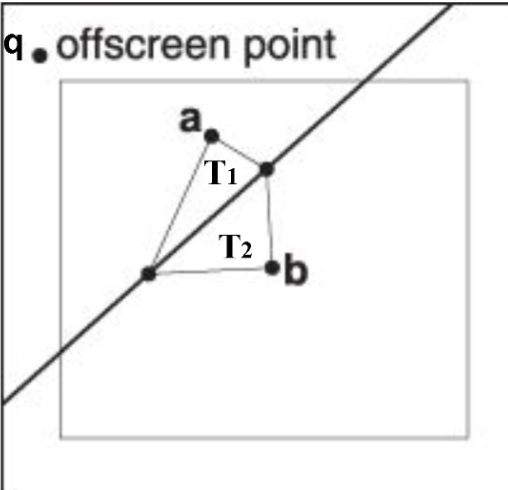
\includegraphics[width=.3\linewidth]{rasterize-triangle-edge.png}

\textbf{Non-overlapping Triangles sharing edges:} We want to ensure no-double drawing.
Assume $T_1, T_2$ share one edge. Let $a$ be the vertex of $T_1$ not along this edge. Let $b$ be the coresponding vertex in $T_2$.
Choose offscreen point $q$.

$T_1$ should be responsible of drawing the edge if $q$ falls on the same side of the edge as $a$. Likewise for $T_2$ and $b$.


\textbf{Proper Perspective Attribute Attribution}: How we set up the above code leads to incorect attribute interpolation when taking perspective into account.
This is because we are interpolating on the 2d projection of the triangle and not considering the distace of the 3d space.

We can interpolate using the following code, which scales based on a scaling metric.

\begin{lstlisting}[language=C++]
float Rs = 60*(R0/w0) + b1*(R1/w1) + b2*(R2/w2);
float Gs = b0*(G0/w0) + b1*(G1/w1) + b2*(G2/w2);
float Bs = 60*(B0/w0) + b1*(B1/w1) + b2*(B2/w2);
float Is = b0*(1/w0) + b1*(1/w1) + b2*(1/w2);
float R = Rs / Is;
float G = Gs / Is;
float B = Bs / Is;
\end{lstlisting}


\textbf{Anti-Aliasing}\\
\textbf{Supersample: }Screen Goal is 256x256. We instead render x4, meaning we actually render a 1024x1024 image. Each highresolution pixel is considered a \textbf{fragment}.
Then, on scale down, we can average the 16 virtual pixels into 1 screen pixel.
Can use box filter or a gaussian filter.\\
\textbf{Multisample: }
Screen goal is 256x256. We still rasterize for a higher resolution, but fragment (triangle) colour computation is only calculated once.
Then, we sample $n$ times from the pixel area, averaging the samples to get the true pixel colour.
\textbf{Fragments} here are each dot on a pixel.

% 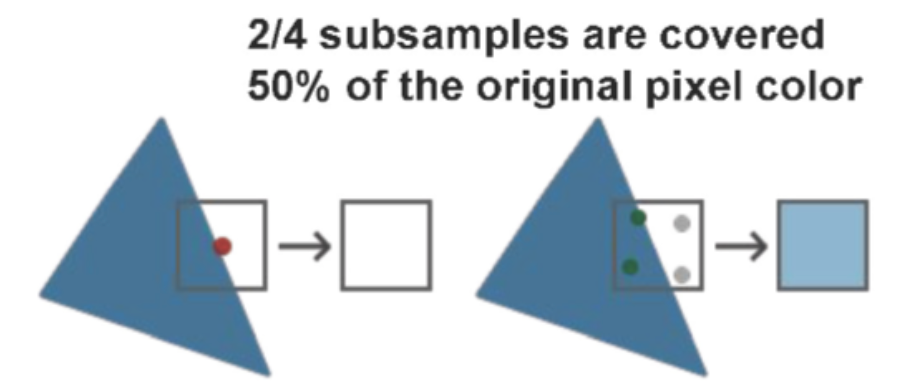
\includegraphics[width=.5\linewidth]{multi-sampling.png}
\section{Pipeline}

\subsection{Application}
\textit{Main Program}
Runs on CPU
Defines geometry vertex positions, normals, texture coords, colours, etc.
Sets up camera position, orientation, projection volume
Sets screen size

Copies data to GPU

\subsection{Vertex Shader}
\textit{Per-vertex Computation}
No transformation: Simply assigns input to output (pass-through shader)
Transforming vertex: Apply \(M_{proj} M_{cam} M_{model}\) to input
Shading: determines vertex color (Gouraud)

GPU performs parallel processing on each vertex

\subsection{Culling}
\subsubsection{Backface Culling}
Removes primitives facing away from camera
Look at face normal / right hand rule,
face normal points in same direction as face.

\subsubsection{View Frustrum Culling}
Removes geometries outside view volume.
6 planes: near, far, left, right, top, bottom.
Plane function is
\(
f(p) = n \cdot (p - a)
= n \cdot p + n \cdot a
= n \cdot p + D
= 0
\)
\textbf{Test if outside view volume}
Take bounding box of object, e.g. a sphere with centre c, radius r.
Check \(f(c)\), \(c\)'s signed distance to plane, see if it intersects or is within frustrum.

\subsubsection{Clipping}
View volume cuts primitive to avoid drawing out of bounds

\textbf{Clipping a Line}
\textit{Plane Function}:
\(f(p) = n \cdot p + D\) or \(f(p) = n \cdot (p - c)\), \(p\) is some point,
\(n\) is the normal, \(D\) is a known const, $c$ is a known point on the plane. If $f(p) = 0$, then $p$ is on the plane.

\textit{Line Function}:
\(p(t) = \mathbf{a} + t (\mathbf{b} - \mathbf{a})\)

\textit{Intersection Point}
Plug \(p\) into plane function \(f(p) = n \cdot (\mathbf{a} + t(\mathbf{b} - \mathbf{a})) + D = 0\)
Solve for \(t = \frac{n \cdot \textbf{a} + D}{n \cdot (\textbf{a} - \textbf{b})}\)

\textbf{Clipping a Triangle}
\begin{figure}[!ht]
    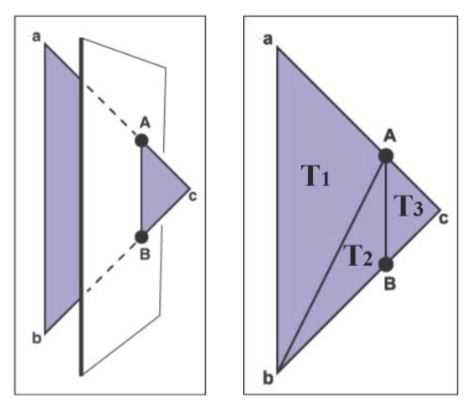
\includegraphics[width=\linewidth]{triangle-clipping.png}
\end{figure}

\textit{Plane Function}:
Same as above

\textit{Intersection}:
Assume \(a, b\) is on one side, \(c\) is on the other side
Compute intersection points \(\mathbf{A}, \mathbf{B}\) using line clipping method.

\textit{Split Triangle}
\(\mathbf{T}_1=\triangle abA, \mathbf{T}_2=\triangle bBA, \mathbf{T}_3\)

\textit{Throw Away}
If \(f(c) \geq 0\), keep \(T_3\); if \(f(c) < 0\), keep \(\mathbf{T}_1, \mathbf{T}_2\)

\textit{Special Case}
Handle zero-area triangles

\section{Depth Testing}

We need to order object rendering so things closer to camera appear `ontop' of things futher away.
Multiple primities can occupy the same fragment.

\textbf{Painter's Algorithm:} Sort primitive by their depths, draw primitives far to near. \textit{Drawbacks:} Sorting is slow, many writes to buffer
Occlusion cycle: cases where no correct order appears correct


\textbf{Color and Z Buffer} Two buffers, one for colour and one for depth. 
Draw primitives as they come in (no sorting), 
check z buffer (inited with $\infty$). 
If the primitive's depth is closer to the camera than what is there (smaller), update the z buffer and override the colour buffer.

\textbf{Z Fighting:} is caused by two primitives sharing the same z value. There are $2^n$ distinct values that $z$ can be, where $n$ is the number of bits for the depth value.
\textit{Precision Formula}:
\(
\text{precision} = (z_{far} - z_{near}) / 2^b
\)
We want \(\text{precision} < \text{max difference between z values}\)
\textit{Mitigation Tactices}: Good near far planes, objects not too close together.


\textbf{Transparency / Alpha}
We can define a primitive's Transparency as $\alpha \in [0, 1]$, color now is RGBA.

$src$ is the colour we want to write, $dest$ is the colour existing in the buffer.

\textbf{Over Operation:} is defined as $\alpha_{src}C_{src} + (1-\alpha_{src})C_{dest}$.
This keeps buffer alpha after the operation=1.

\textbf{Post-multiplication}
Set dest rgb using the over operation. $C_{src} = (R,G,B)$.

\textbf{Pre-multiplication}
Premultiplied alpha has $C_{src}$ already multiplied together with $\alpha_{src}$ when calculating the blending.
Thus, we set dest rgb. $C_{src} = (R\alpha_{src},G\alpha_{src},B\alpha_{src})$.

$C_{dest} = C_{src} + (1-\alpha_{src})C_{dest}$.

\textbf{Alpha and Depth Test}

Zbuffer does not care if the fragment has Transparency -- Fragments are not ordered. However- \textbf{ORDER matters when dealing with transparency!}. 
Thus, We draw all opaque objects first using the depth buffer, then use painters algorithm to draw transparent objects.

\section{Mesh}
Manifold intuition:
Mesh is ``watertight'',
``a small neighborhood around any point could be smoothed out into a bit of flat surface''
\textbf{Manifold:} Every edge is shared by exactly two triangles. Every vertex has a single, complete loop of triangles around it.
\textbf{Manifold with Boundary:} Every edge is used by either one or two triangles. Every vertex connects to a single edge-connected set of triangles.

Manifold useful for 2d regular grid,
better control of neighboring topology,
consistent triangle orientation.

\textbf{Implicit vs Explicit}: Explicit Defines 3D geometry via vertices, edges, and faces. Implicit Defines 3D geometry via a mathematical function

\textbf{Pros of Explicit Representation:} Efficient rendering, direct manipulation, widely supported.
\textbf{Cons of Explicit Representation:} Memory-heavy, complex storage, explicit connectivity needed.
\textbf{Pros of Implicit Representation:} Compact for complex shapes, smooth surfaces, ideal for Boolean operations.
\textbf{Cons of Implicit Representation:} Costly rendering, harder to edit, requires function evaluation.

\textbf{Euler's Formula:} $V - E + F = 2(1 - g) \approx 0$
Where $F$ is \# of triangles,
$E$ is \# of edges,
$V$ is \# of verticies,
$g$ is genus (\# of holes in surface)
Each edge is used 2x, each triangle uses 3 edges, $2E = 3F$.
$F = 2V, E = 3V$.

\subsection{Mesh data structures}
\subsubsection{Separate Triangles (Triangle Soup)}
It's just an unorganized list of triangles.
Storage cost: $F \cdot 3 \cdot 3 \cdot 4 = 72 \cdot V$ (72 bytes per vertex)
(F triangles, 3 vertices, 3 vector components, Euler formula)

\subsubsection{Indexed Triangle Mesh}
Store list of vertices, list of triangle indices separately.
Allows for deduplicating vertices, decoupling vertex positions from connectivity. (Blendshapes)
Vertices in Bytes: $V \cdot 3 \cdot 4 = 12 V$
Triangles in Bytes: $F \cdot 3 \cdot 4 = 12 F \approx 24 V$
Total in bytes is $12V + 24V = 36V$ (36 bytes / vertex)

\subsubsection{Triangle Fans}
List of vertices, list of fan arrays
First vertex is center. Each following adjacent pair forms a triangle with center coord.

\subsubsection{Triangle Strips}
Three adjacent vertices form a triangle.
Streaming in new vertex.
Forget the oldest vertex.
Swap order of remaining two vertices for every other triangle (don't swap 0th, swap 1st, etc.)

Storage for fans and strips, vertices is $12 V$ (same as ITM),
triangle fans / strips array is $(F + 2) \cdot 4 = 4F + 8 \approx 8V + 8$.
Total is $12 V + 8 V + 8 \approx 20V$ (20 bytes / vertex)

\subsubsection{Triangle-Neighbor Structure}
Connectivity info stored in Triangle.
3 vertices in order, 3 neighboring triangles in sync with v.
The side from $v[i]$ to $v[x]$ belongs to triangle $i$.
Efficient for adjacency-based operations like smoothing, traversal, and region-growing,
and is memory-efficient for static meshes.
Lacks granularity at the edge or vertex level,
making it unsuitable for operations requiring detailed connectivity or dynamic topology changes.
\textbf{Traverse triangles of vertex v.}
Pick any triangle t connects to v.
Find the neighboring triangle correspoinding to v.
Set t to be neighboring triangle.
Loop until we get back to the start.
\textbf{Storage:}
Triangles: $F \cdot (3 + 3) \cdot 4 = 24F$
Vertex: $V \cdot (1 + 3) \cdot 4 = 16V$
Total is $24F + 16V \approx 48V + 16V \approx 64V$ (64 bytes / vertex)

\subsubsection{Winged-Edge Structure}
Connectivity information stored in edge.
2 vertices of edge, head and tail
2 neighboring triangles, left and right
prev and next edges in left triangle,
ditto for right triangle.
Left tri contains lprev, lnext, [tail-head].
Right tri contains rprev, rnext, [head-tail].
\textbf{Traversal given vertex:}
Follows prev (aka always pick the edge to the left),
edges around v visited in ccw order.
\textbf{Traversal given face:}
Stays on the side where face is,
visit edges of face in ccw order.
\textbf{Storage}
Edge in bytes: $E \cdot 8 \cdot 4 = 32E$ (8 references, we can remove prevs to save space and just do 2 nexts instead)
Triangle in bytes: $F \cot 1 \cdot 4 = 4F$
Vertex in bytes: $V \cdot (1 + 3) \cdot 4 = 16V$ (1 edge ref, xyz)
Total: $32E + 4F + 16V \approx 96V + 8V + 16V \approx 120V$.

\subsubsection{Winged-Edge and Half Edge Diagram}
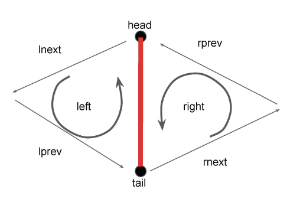
\includegraphics[width=.3\linewidth]{winged-edge.png}
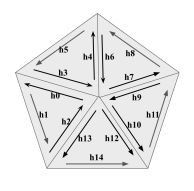
\includegraphics[width=.3\linewidth]{half-edge.png}

\subsubsection{Half-Edge Structure}
Halfedge:
VertexRef v (vertex half-edge points to)
TriangleRef t (triangle that the halfedge is on)
HalfEdgeRef prev, next (
HalfEdgeRef pair

\textbf{Storage}
Half-edge in bytes: $(E \cdot 2) \cdot 5 \cdot 4 = 40E$
Triangle in bytes: $F \cdot 1 \cdot 4 = 4F$
Vertex in bytes: $V \cdot (1 + 3) \cdot 4 = 16V$
Total: $40E + 4F + 16V \approx 120V + 8V + 16V \approx 144V$

\section{Mesh Editing}

Edge Flip \quad\quad\quad\quad\quad\quad\quad\quad\quad Edge Split

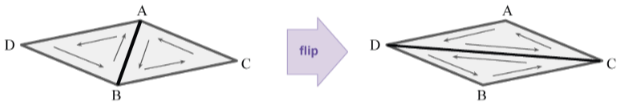
\includegraphics[width=.45\linewidth]{edge-flip.png}
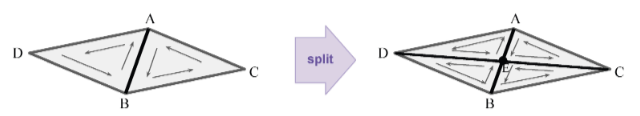
\includegraphics[width=.45\linewidth]{edge-split.png}

Edge Collapse

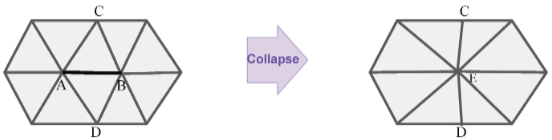
\includegraphics[width=.45\linewidth]{edge-collapse.png}
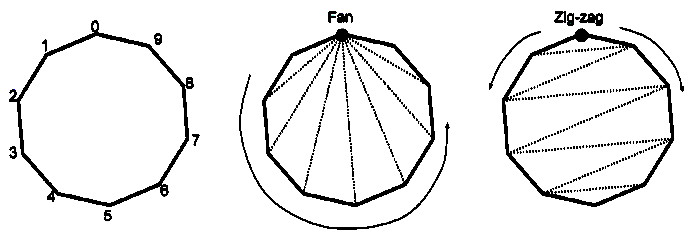
\includegraphics[width=.45\linewidth]{triangulation.png}

\subsection{Subdivision}
\textbf{Split:} insert new vertices
\textbf{Interpolate:} recompute positions for original and new vertices

\subsection{Loop Subdivion}
New vertices are added at positions of weighted sum of original vertices on neighboring faces.
For interior, $v = 3 \cdot (A + B) / 8 + (C + D) / 8$ where $v$ lies on the edge between $A$ and $B$.
For boundary, $v = (A + B) / 2$.
Original vertices are reweighted based on original neighboring vertices.
$v_{new} = (1 - n \beta) v_{original} + \beta \sum v_{neighbor}$.
Where $n$ is $v$'s degree.
Implementation: split each triangle edge in any order, flip any edge connecting a new and an original vertex.

\subsection{Linear Subdivision}
Input: m-gon. Output: m quads per m-gon.
Face vertex: average of face corner vertices
Edge vertices:  average of two vertices at ends of edge
Vertex from original mesh: keep original.

\subsection{Catmull-Clark Subdivision}
Face vertex position is average of all original face corner vertex positions
Edge vertex position is average of two end vertices and two face vertices
Original vertex position is change according to
$\frac{Q + 2R + (n-3)S}{n}$
Where $Q$ is average position of face vertices neighboring $v$,
$R$ is average position of all edge vertices connected to $v$,
$S$ is original vertex position of $v$,
$n$ is $v$'s degree.

\subsection{Quadric Error Simplification}
Given a plane $ax + by +_ cz + d = 0$,
let \\ $u = \begin{bmatrix}
    a \\ b \\ c \\ d
\end{bmatrix}$
then, $K_{plane} = \begin{bmatrix}
    a^2 & ab & ac & ad \\
    ab  & b^2 & bc & bd \\
    ac & bc & c^2 & cd \\
    ad & bd & cd & d^2 \\
\end{bmatrix}$
$K_{vert} = \sum K_p \forall \text{adj. planes}$
and $K_{edge-ij} = K_i + K_j$.
The metric to minimize is $o^T k_{ij} o$,
the distance from $o(x, y, z)$ to edge $ij$.
To solve,
$
\begin{bmatrix}
    x \\ y \\ z
\end{bmatrix}
=
\begin{bmatrix}
    k_{11} & k_{12} & k_{13} \\
    k_{21} & k_{22} & k_{23} \\
    k_{31} & k_{32} & k_{33} \\
\end{bmatrix}^{-1}
\begin{bmatrix}
    -k_{14} \\ -k_{24} \\ -k{34}
\end{bmatrix}
$

\subsection{Isotropic Remeshing}
Let $L$ be mean edge length of input mesh
If an edge is too long ($>4/3L$), split it
If an edge is too short ($<4/5L$), collapse it
If flipping an edge improves degree of neighboring vertices, flip it:
Deviation is $\sum_A^D|deg(X) - 6|$, if deviation drops after a flip then flip the edge.
Move vertex positions towards average of their neighbors:
For vertex $P$, computer centroid $C$ of all neighbours.
Movement vector is $v = C - P$, move by $1/8 v$.
Ignore movement in normal direction N by using $v - N(N \cdot v)$
Vertex normal is weighted sum of face normals
$N = \sum_{neighbor triangle t} t.area * t.normal = \sum cross(t.edge1, t.edge2)$
Then normalize

\subsection{Blendshapes}
This is trivial, just calculate offsets with $o_i = (bs_i - base)$,
and build final blendshape with $shape = base + \sum w_i \cdot o_i$.

\section{Texture}

\subsection{Projections}
\subsubsection{Planar Projection}
$
\begin{bmatrix}
    u \\ v \\ * \\ 1
\end{bmatrix}
= M_t \begin{bmatrix}
    x \\ y \\ z \\ 1
\end{bmatrix}
$
Where $M_t$ is affine transformation matrix.

\subsubsection{Spherical Coordinates}
$
u = \frac{[\pi + atan2(y, x)]}{2 \pi} \quad (atan2(...) = \phi)
$
$
v = \frac{[\pi - acos(\frac{z}{\sqrt{x^2 + y^2 + z^2}})]}{\pi} \quad (acos(...) = \theta)
$
$atan2 \in [-\pi, \pi], acos \in [0, \pi]$
Has issues for oddly shaped objects (eg cylinders),
areas with large r are sparse vs areas with small r.

\subsubsection{Cylindrical Coordinates}
$
u = \frac{[\pi + atan2(y, x)]}{2\pi} \quad atan2(...) = \phi
$

$
v = \frac{1 + z}{2}, z \in [-1, 1]
$

\subsubsection{Cubemap (Skybox)}
$
u = \frac{1 + y / |x|}{2}, v = \frac{1 + z / |x|}{2} \text{ where } |x| > |y|, |x| > |z|, x > 0
$

\subsubsection{Seams}
If we don't handle seams, wrapped texture will have
triangles ``wrap'' across the whole texture, making a bad seam where the texture should repeat.
Instead, we duplicate the vertices on the left and right edges, such that the left seam's edges only apply to the triangles on it's right,
and the right seam's edges only apply to the triangles on it's left.

\subsection{Barycentric Interpolation}
Get barycentric of $p$ inside triangle $b1, b2, b3$.
Interpolate $uv$ for $p$:
$u_p = b1 \cdot u_a + b_2 \cdot u_b + b_3 \cdot u_c$

\subsection{Sampling}
\textbf{Nearest:} Self-explanatory
\textbf{Bilinear:} Also kinda self-explanatory, see interpolation on page 1.
\subsection{Wrapping}
UV is in range [0,1], deals with how to handle stuff outside of range.
Clamp: use edge colour for stuff outside range
Tile: repeatedly sample the texture (loop it)

\subsection{Mipmap}
Take the longest length $l$,
the mipmap level to take is $\log_2 l$.
Level 0 is base image, each texel in level $k$ image is avg of $2^k \times 2^k$ texels in original texture.

\subsection{Maps}
\textbf{Diffuse Map:} Stores colours, RGB
\textbf{Normal Map:} Stores normal vectors to determine bounce directions, 3 channels
\textbf{Displacement Map:} Changes vertex positions by $x$ amount in the normal direction, 1 channel, slow
\textbf{Bump Map:} Scales normals by $x$ amount in the normal direction, does not change vertex positions, 1 channel, fast
\textbf{Shadow Map:} Stores distance to first point hit by each light in a preprocessing step (z buffer).
During rendering, calculate each fragment's distance from light and illuminate it if it's less than or equal to the stored value.
Otherwise, it is in shadow.

\section{Light}
2D Angle: $l / r (radians)$
3D Angle: $A / r^2 (steradians)$

\textbf{Radiant Flux:} Power (\unit{\watt})
\textbf{Irradiance:} Power per square unit of area (\unit{\watt\per\square\metre})
\textbf{Radiance:} Power per square unit of area per direction (\unit{W.m^{-2}.sr^{-1}})
\textbf{Radiant intensity:} Power per direction (\unit{W.sr^{-1}})

Point light irradiance: $E = \frac{\Phi}{4 \pi r^2}$
Fractional area on sphere $\frac{2 \pi (1 - cos \varphi)}{4 \pi}$
where $\varphi$ is cone half-angle
$F_{att} = \frac{1.0}{K_c + K_I \cdot d + K_1 \cdot d^2}$
Spotlight soft edges, inner cutoff $\varnothing$, outer cutoff $\gamma$


\section{Material}
$$
L(P, \omega_0) = L_e(P, \omega_0) + \int_\Omega f_r(P, \omega_i, \omega_0) L_i(P, \omega_i) \cos \theta_i\ d \omega_i
$$
$L(P, \omega_0)$: Outgoing radiance @ $P$ in $\omega_0$ direction
$L_e(P, \omega_0)$: Emitting light radiance @ $P$ in $\omega_0$ direction if light source, else 0
$\int_\Omega$: Sum over all incoming direction
$f_r(P, \omega_i, \omega_0)$: How incoming light at point $P$ in $\omega_i$ direction is reflected in $\omega_0$ direction
$L_i(P, \omega_i) \cos \theta_i$: Incoming light radiance at point $P$ in $\omega_i$ direction, weighted by $\cos \theta_i$.

\subsection{Diffuse}
\textbf{Diffuse OpenGL:} \\
light direction $l = light_{pos} - vertex_{pos}$ \\
\verb|diffuse_light_clr * diffuse_mat_clr * max(0, dot(n, l)) / r^2|
($n \cdot l = \cos \theta$)

\subsection{Specular}
Exponent: lower $p$ is more diffused, higher $p$ is more reflective
\textbf{Specular OpenGL:}
Find reflected light direction \\ $r = -l + 2(l \cdot n) n$.
Vertex direction $P_p$, camera position $P_c$,
find view direction \\ $v = norm(P_c - P_p)$.
Color on object = \\ \verb|specular_light_clr * specular_material_clr * max(0, dot(v, r)^p)|

\subsection{Phong}
Phong shading is the sum of ambient, diffuse, and specular lighting. (Multiplied by $I/r^2$ to simulate light falloff)
$
L(P, v) = [k_a + k_d \cos \theta + k_s (\cos \rho)^p] \cdot \frac{I}{r^2} = [k_a + k_d (n \cdot l) + k_s (r \cdot v)^p] \cdot \frac{I}{r^2}
$
In OpenGL: ambient_light_clr * ambient_material_clr + diffuse_light_clr * diffuse_material_clr * max(0, n$\cdot$l) + specular_light_clr * specular_material_clr * max$(0, v\cdot r)^p$

\subsection{Blinn-Phong}
Instead of using the viewing angle for specular, we use the half-vector $h$, which is halfway between the view and light directions. ($\frac{l+v}{\vert\vert l+v \vert\vert}$).
When adding specular it is now specular_light_clr + specular_material_clr * max$(0,n\cdot h)^p$. \

Blinn-Phong can produce bad results when $r \cdot v$ is negative, but $n \cdot h$ is positive. In this case, Blinn-Phong will be too bright.
\includegraphics[width=.5\linewidth]{phong\_vs\_blinn-phong.png}


\subsection{Gouraud}
Instead of computing color based on lighting in the \textit{fragment shader step},
Gouraud does it using \textit{vertex positions} using vertex colors during the vertex shader.

\section{Ray Tracing}
Ray representation: $r = o + td$

\subsection{Ray Gen}
left, right, top, bottom are coords defining bounds of view volume.
view volume is $n_x$ px wide, $n_y$ px high.

\textbf{pixel(i, j) $\to$ (u, v, w) coord}
$u = left + (i + 0.5) * (right - left)/n_x$;
$v = bottom + (j + 0.5) * (top - bottom)/n_y$;
$w = -fl$
\subsubsection{Perspective}
$o = e$ (e is camera coords);
$d = u \vec{u} = v \vec{v} - fl \vec{w}$ (uvw is camera view coords, w is away from looking location)

\subsubsection{Orthographic}
$o = e + u \vec{u} + v \vec{v}$
$d = -\vec{w}$


\subsection{Ray-Object Intersection}
\subsubsection{Sphere}
Point $\mathbf{p}$ on ray: $\mathbf{p} = \mathbf{o} + t\mathbf{d}$
Point $\mathbf{p}$ on sphere centred at $\mathbf{c}$ with radius $R$: $(\mathbf{p} - \mathbf{c}) \cdot (\mathbf{p} - \mathbf{c}) - R^2 = 0$
Intersection points: $(\mathbf{o} + t\mathbf{d} - \mathbf{c}) \cdot (\mathbf{o} + t\mathbf{d} - \mathbf{c}) - R^2 = 0$
Solve for $t$:
$t = \frac{-\mathbf{d} \cdot (\mathbf{o} - \mathbf{c}) \pm \sqrt{(\mathbf{d} \cdot (\mathbf{o} - \mathbf{c}))^2 - (\mathbf{d} \cdot \mathbf{d}) \cdot ((\mathbf{o} - \mathbf{c}) \cdot (\mathbf{o} - \mathbf{c}) - R^2)}}{\mathbf{d} \cdot \mathbf{d}}$
Normal $\mathbf{n}$ at hit point $\mathbf{p}$:
$(\mathbf{p} - \mathbf{c}) / R$

\subsubsection{Triangle}
Representation of $\mathbf{p}$:
$\mathbf{p} = \alpha \mathbf{A} - \beta \mathbf{B} + \gamma \mathbf{C} = (1 - \beta - \gamma) \mathbf{A} + \beta \mathbf{B} + \gamma \mathbf{C}$
Point $\mathbf{p}$ on triangle $\mathbf{ABC}$:
$\mathbf{p}=\mathbf{A} + \beta (\mathbf{B} - \mathbf{A}) + \gamma(\mathbf{C} - \mathbf{A})$
Intersection point:
$\mathbf{o} + t \mathbf{d} = \mathbf{A} + \beta(\mathbf{B} - \mathbf{A}) + \gamma(\mathbf{C} - \mathbf{A})$
$
\begin{bmatrix}
    \beta \\ \gamma \\ t
\end{bmatrix}
=
\begin{bmatrix}
x_A - x_B & x_A - x_C & x_d \\
y_A - y_B & y_A - y_C & y_d \\
z_A - z_B & z_A - z_C & z_d \\
\end{bmatrix}^{-1}
\begin{bmatrix}
    x_A - x_o \\
    y_A - y_o \\
    z_A - z_o \\
\end{bmatrix}
$

\subsubsection{Rectangle (this is for xy plane)}
Point p on axis aligned rect: $z_p = k$
Intersection: $z_p = z_o + t z_d = k$
Solve for t: $t = (k - z_o) / z_d$
Plug back, check $x_p \in [x_0, x_1], y_p \in [y_0, y_1]$ so it's in rect.

\subsection{Shading}
\textbf{Lambertian:} $res = diffuse \cdot I \cdot max(0, n \cdot l) / (dist^2)$
diffuse is obj colour, I is light colour, dist is abs(lpos - p), l is (lpos - p) / dist.
\textbf{Specular:}
$l = (lpos - p) / |lpos - p|$;
$h = (l + (-d)) / |l + (-d)|$;
$res = specular \cdot I \cdot max(0, pow(h \dot n, 5))$

\textbf{Shadows}
shadow_ray: $p + t l$
dist: $|lpos - p$
$t \in [\epsilon, dist]$
if $t < dist$ then it hit an object before the light and thus is in shadow.

\section{Extra}
\subsection{Spatial Data Structure}
Used to quickly locate objects in space\
\textbf{Binary space partition (BSP)}
While every object is not in its own region, split the space in half\
Hyperplanes; for higher dimensions (3D), splits space similarly to Binary space partitioning. Splitting hyperplanes can be completely arbitrary
\textbf{Autopartition}
Candidates for splitting are based on input primitives; when we have inputs, we just extend the planes further to split space.\
\textbf{K-D Tree} \
K means number of dimensions. 2D example: we split along the median of the X values, then we split along the Y medians of the 2 resulting partitions, then X, etc, etc. until every point is a median.
\textbf{Octree / Quadtree}
\textbf{Octree}: Divide 3d space into 8 quadrants, keep dividing the resulting space until each has <=1 point in each cell
\textbf{Quadtree}: Divide 2d space into 4 quadrants, keep dividing until each space has <=1 point in each cell


\subsection{Curves}

\subsubsection{Desirable Properties}
\textbf{Continuity:} $n^{th}$ derivative remains the same. $C^0$: lines connect,
$C^1$: velocity remains the same,
$C^2$: acceleration remains the same.
\textbf{Locality:} Local - one control point only impacts a small piece of the curve.
Global - one control point impacts the shape of the whole curve
\textbf{Interpolation:} Interpolation - Curve passes through all control points.
Approximation - Curve does not pass through all control points,
but control points determine curve.
Ideally we want at least $C^2$ continuity,
locality, and interpolation.

\subsection{Disadvantages of Single Piece Polynomial Curves}
\begin{itemize}
    \item Lack of locality. Changes to points affect the whole curve.
    \item Runge's Phenomenon: Oscillation with polynomial interpolation causes increasing wiggles and overshoots near the outer control points.
\end{itemize}


\subsection{Cubic Spline}
\begin{itemize}
    \item Defined as $a_0 + a_1t + a_2t^2 + a_3t^3$.
    \item Properties: Locality, $C^2$ continuity, Interpolates the control points.
\end{itemize}

\subsection{Cardinal Spline}
\begin{itemize}
    \item Defined by $n+1$ control points.
    \item Uses positional and derivative constraints.
    \item Derivatives calculated using a tension constant $c$ and the positions of neighboring points:
    \begin{align*}
        F(0) &= p_1 \\
        F'(0) &= (1-c)(p_2 - p_0)/2
    \end{align*}
    \item Catmull-Rom is a special case of Cardinal Spline where $c = 0$, implying $ F'(0) = p_2 - p_0)/2$
\end{itemize}

\subsection{Properties of Different Curve Types}
TC = Total Constraints
\begin{center}
\begin{tabular}{|l|c|c|c|}
    \hline
    Curve Type & Continuity & Locality &  TC \\
    \hline
    Single Polynomial  & $C^n$ & Global & -- \\
    Hermite Cubic  & $C^1$ & Local & $4n$ \\
    Cardinals & $C^2$ & Local & $4n$ \\
    Catmull-Rom  & $C^2$ & Local & -- \\
    \hline
\end{tabular}
\end{center}

\subsection{Deriving Spline Basis for Cubic Curves}
\begin{itemize}
    \item Follow the process of deriving Hermite basis.
    \item Apply the same methodology to derive the basis for Catmull-Rom splines.
\end{itemize}

Recall the cubic functions
$f(t) = a_0 + a_1t + a_2t^2 + a_3t^3$ and
$f`(t) = a_1t + a_2t + 3a_3t^2$.

We also have the Hermite equations for a segment: $f(0) = p_0 = a_0, f(1) = p_1 = a_0 + a_1 + a_2 + a_3, f`(0) = p_2 = a_1, f`(1) = p_3 = a_1 + 2a_2 + 3_a3$. Name $p$ as the set of parameters.

We can rewrite set of equations as $p = Ca$, where $C$ is a matrix of 0's and 1's.

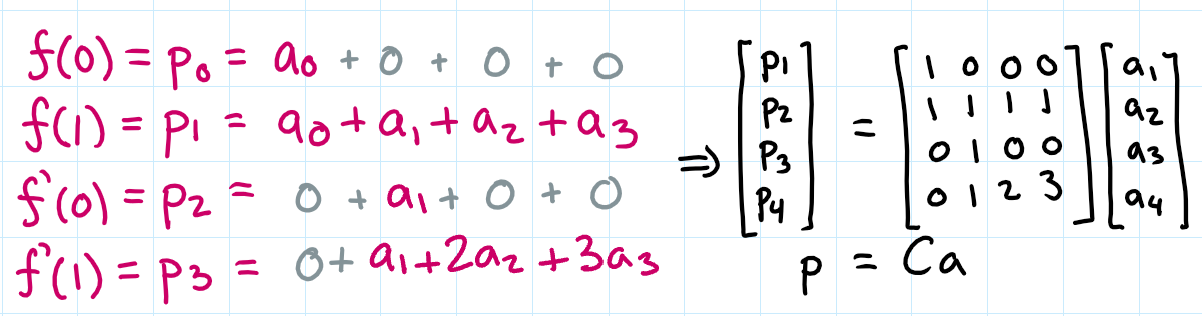
\includegraphics[width=0.3\linewidth]{
curve-basis-soe.png}

Take $p=Ca$, rearrange $C^{-1}p=a$.

Now we have expressions for $a_i$ in terms of $p$. We can replace all $a's$ in the original $f(t)$ to be in terms of $p$. Rearrange that to collect like terms of $p$, we get a basis.

Hermite Basis:
$f(t) = p_1(2t^3 - 3t + 1) + p_1(-2t^3+3t^2) + p_2(t^3-2^2 + t) + p_3(t^3-t^2)$

Where $p_1 = p_0, p_2 = p_1, p_3 = p^`_0, p_4 = p^`_1$


\subsection{Deriving Bezier Basis}

Depending on the bezier `degree' $n$, we can calculate it via $b_i,n = \frac{n!}{i!(n-i)!}(t^i)(1-t)^n-i$.

$b_0,3 = (1-t)^3$
$b_1,3 = t(1-t)^2$
$b_2,3 = t^2(1-t)^1$
$b_3,3 = t^3$


\subsection{Computing Positions on the Curve Using Spline Basis}
\begin{itemize}
    \item Given user constraints, compute positions using the basis functions $b$ and constraints $p$:
    \begin{align*}
        F(t) = p_0b_0(t) + p_1b_1(t) + p_2b_2(t) + p_3b_3(t)
    \end{align*}
\end{itemize}

\subsection{Computing Positions on Bezier Curves Using the de Casteljau Algorithm}
Define the `control polynomial', then connect the intersections between the points.

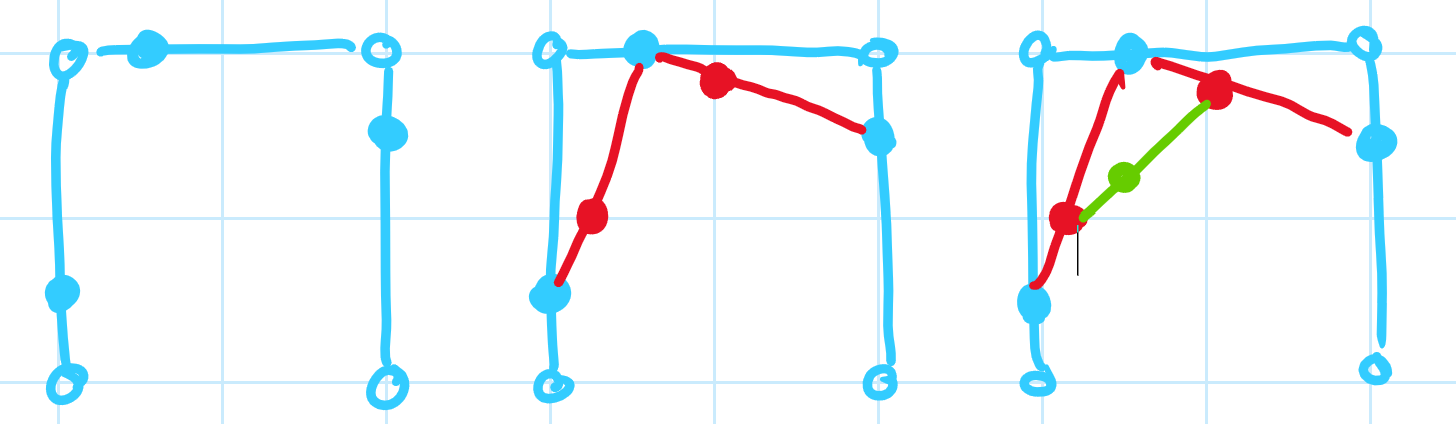
\includegraphics[width=0.3\linewidth]{bezier.png}


\end{multicols*}

\end{document}
